% Engineering Methods
%#cvicenie - opytat sa na cviceni
%ULOHA - treba spravit

\documentclass[11pt ,english,a4paper]{article}

\usepackage[english]{babel}
\usepackage[IL2]{fontenc}
\usepackage[utf8]{inputenc}
\usepackage{graphicx}
\usepackage{url}
\usepackage{hyperref}
\usepackage{times}
\usepackage{setspace}

\setstretch{1.5}
\pagestyle{headings}

\title{Efficiency comparative analysis of techniques in misinformation detection in healthcare data\thanks{Semestral project in subject Engineering Methods, ac. year 2023/24, guidance: MSc. Mirwais Ahmadzai}}

\author{Alžbeta Žiarovská\\[2pt]
	{\small Slovak University of Technology in Bratislava}\\
	{\small Faculty of Informatics and Information Technologies}\\
	{\small \texttt{xziarovska@stuba.sk}}
	}

\date{\small 26. september 2023}



\begin{document}

\maketitle
\newpage

\begin{abstract}
\ldots
\end{abstract}
\newpage

\section{Introduction}\label{intro}

In this article I am going to discuss the current situation regarding spread of misinformation in the medical field. This topic is very important in the aftermath of the global COVID-19 pandemic. More specifically I am going to make an analysis and comparison of different misinformation detection methods and their efficiency. During the pandemic we have seen a great rise of misinformation on the Internet, which provide danger to our society or even lives \cite{war18dr}. The main problem in my perception is, that the easy access to all the information on the Internet, which does not necessarily has to be true, can increase fear and anxiety and ultimately lead to the delay of diagnosis and receiving the effective healthcare in case the information are not perceived correctly \cite{wa19sys}. The paradox is, that the machines might actually be the solution, as I am going to discuss various methods to recognize misinformation using technology \cite{chap22unmask}.

I am focusing on comparing fact-checking and machine learning models as s way to find the medical misinformation. The fact-checking can be done manually or automatically which is introduced more deeply in Section \ref{tech:fact} \cite{bar21health}. The other side I am taking a closer look at are machine learning techniques including Naïve Bayes, Support Vector Machine and BERT-based model called Disease Myth Buster \cite{bar21health} \cite{chap22unmask}. I introduce these techniques and compare their efficiency in order to establish which one is the most suitable for a specific situation in healthcare.

In the Section \ref{ter} I am giving a brief introduction into the terminology used in the article.. In the Section \ref{mih} the term misinformation is described, how it differs from disinformation \cite{gu20misinfo}. Also a brief summary of historical development of misinformation spread is given \cite{pos18short}. It is also important to mention affect that medical fake news might have on our lives, which I address as well \cite{who22infodemics}. The last but not least, in Section \ref{tech}, I am taking a closer look at some of the methods used for misinformation recognition. I going to introduce them in a way, that would be easily understandable for all readers and state some of their outputs, so I can compare their effectiveness and possible impact for the future in Conclusion. \ref{conclusion}

\section{Terminology}\label{ter}

\paragraph{Natural language processing} (NLP) is a way for programs to understand language used by humans on daily basis by using various algorithms an limitations \cite{nad11natural}.

\paragraph{Term frequency–inverse document frequency} (TF-IDF) represents a numeric value of how relevant is the specific word for the document in the set of documents. This technique finds its application both in text mining and information retrieval \cite{chr16tfidf}. 

\section{Misinformation in healthcare}\label{mih}

\paragraph{Difference between misinformation and disinformation}
The terms \emph{misinformation} and \emph{disinformation} are much the same, however, a small, but crucial difference can be distinguished. The difference between the two is a intention with which the false information is made accessible to the public and spread. Whilst the misinformation is usually created without direct intention of misleading and spreading false, meaning the person who put the information into the world might not actually know it is not true. On the other hand, disinformation is essentially created to spread false information. An example of such activity can be political propaganda \cite{gu20misinfo} \cite{cook15misinfo}. Even though the terms are not meaning the same, for the purpose of this article they are used as synonyms, because the author's knowledge, whether the information is factual, is negligible in the scope of its false recognition.

\paragraph{Historical development of concept of misinformation}%Lecture topic reaction
As the historical events have shown, the yearn for spreading not true information, either for amusement or with a goal of hurting someone, is old as a humanity itself \cite{bur17history}.%#cvicenie Do I have to cite the general introduction to the paragraph?

The very first use of misconception was spoken, whereas the printing was not found yet. The emperors used to control the information generally believed in order to strengthen their reign and power over the people. \cite{bur17history} In the 16th century the writers have started to create completely false stories and plays in order to offer entertainment, but the drive was not only positive. During the French Revolution a rumor (in France called \emph{canard}) was used to discredit the queen Marie Antoinette, which doubtlessly did not help her in the later events of the French Revolution. \cite{bur17history} 

Later, when the mass media took their place, the misleading was often used in order to change the opinion of the public during the times of war. For example during the World War II the Nazi propaganda was reaching the peaks of political propaganda ever. \cite{pos18short}

As we have entered the era of the internet, everybody can contribute to the chain of communication and share their own truth, whether with or without the intention of doing harm. The rise of the \emph{hoax} is enormous and numerous fake websites were created.\cite{bur17history} The ways of popularizing the misinformation has changed, as new inventions were developing, and so did the way of fighting them. Nowadays the information revolution by the Internet has brought many ways of spreading false information, but the way of their detection is not yet perfectly defined and therefore there is need for effective adaptive mechanisms.

\paragraph{Health care misinformation}

\cite{wa19sys}\cite{cook15misinfo}
%Moreover,Internet content is fast becoming a replacement for expert advice,with a majority of Americans looking online for health information. However,numerous analyses of online content have found that a significant proportion of websites provide inaccurate medical information. \cite{cook15misinfo}
%and tobacco manufacturers have promoted misinformation about the public health impacts of smoking. \cite{cook15misinfo}

\paragraph{Societal context}%Lecture topic reaction
\cite{who22infodemics} page 8 \cite{wa19sys}


\section{Misinformation recognition techniques} \label{tech}

\subsection{Fact-checking technique} \label{tech:fact}
The process of fact-checking is used to distinguish, whether the specific claim is based on facts. This technique is usually used in a field of journalism \cite{alh18fact}.
There are two basic types of fact-checking to be differentiated:\cite{vla14fact} 
\begin{itemize}
\item Manual fact-checking
\item Automatic fact-checking
\end{itemize}
In subsection \ref{tech:fact:man} and \ref{tech:fact:auto} both of these will be introduced briefly.

\subsubsection{Manual fact-checking}\label{tech:fact:man}
Manual fact-checking is important process when we find some potentially false information on the Internet. However, it can be rather time consuming and usually ineffective way of finding factual information when the source is quite complex and contains a lot of detailed information \cite{gu22fact}. I offer a list of some of the basic points that can hold to in order to make the manual fact-checking as effective and quick as possible:
\begin{enumerate}
\item{\emph{Context}} - It is crucial to distinguish, whether the information is meant to be served as a fact to provide information or even to convince, or whether it is supposed to be taken as an exaggeration or sarcasm \cite{alh18fact}.
\item {\emph{Sentimental value}} - The goal of misinformation is often to scare people and spread panic. The difference between ratio of positive and negative in true and false claims is notable. Whilst in true claims the ratio is 71\% of positive words to 29\% of negative words, in misinformation sources this ratio is shifted the other way around with only 38\% of positive words and 62\% of negative words \cite{bar21health}.
\item {\emph{Sources}} - Perhaps the most important step might be to check the original sources of the claim \cite{gra17fact}. Anybody can share anything on the internet, so it is important to check, where does the information originally come from. We might need to look for the trustworthiness of the website or references, where did the author get the information from.
\end{enumerate}
In the figure \ref{f:man_fact} I created a mind map to illustrate the steps in process of manual fact-checking I enlisted in this section.

\begin{figure}[h]
\centering
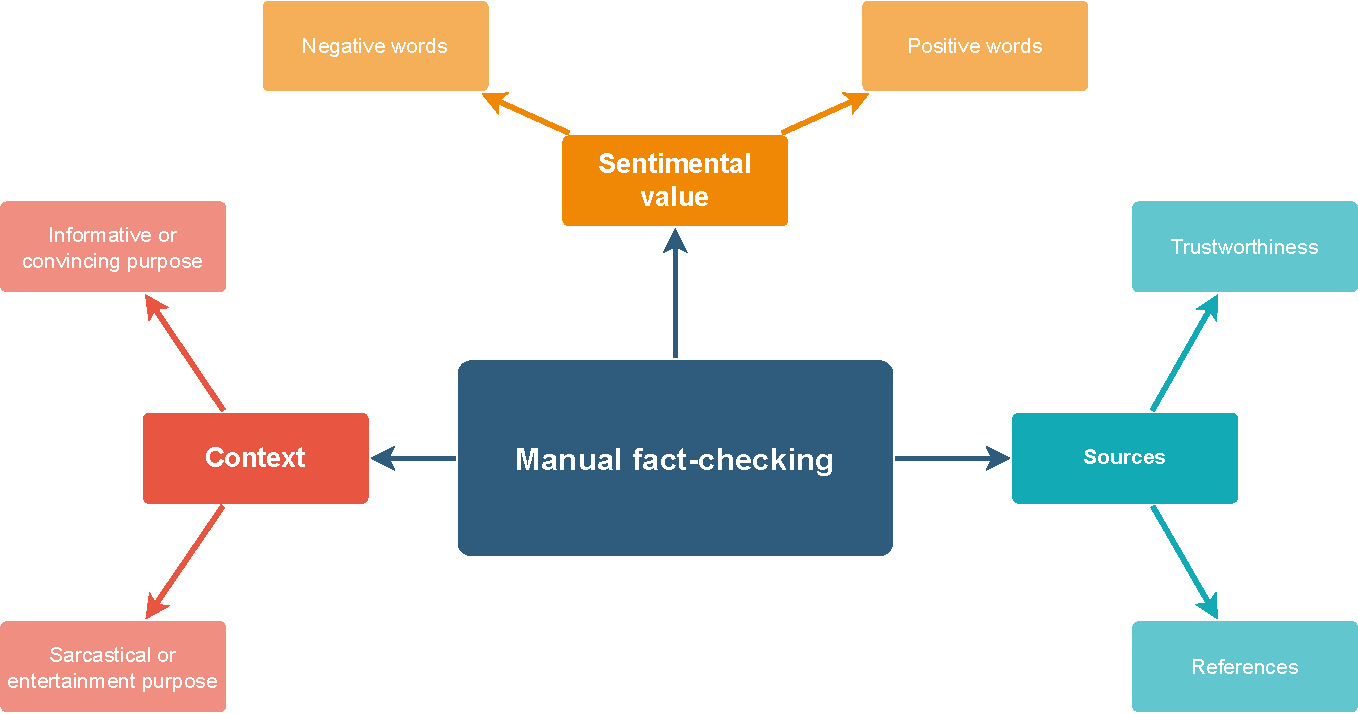
\includegraphics[scale=0.5]{manual_factchecking.pdf}
\caption{Mind map of Manual Fact-checking steps.}
\label{f:man_fact}
\end{figure}

\paragraph{Technology and people}%Lecture topic reaction
%backfire and boomerang\cite{cook15misinfo}
%How can we benefit from manual fact-checking in out everyday lives

\subsubsection{Automatic fact-checking}\label{tech:fact:auto}
%websites FACTCHECK.org,POLITIFACT.comandFULLFACT.org \cite{alh18fact}
\cite{gu22fact}

\subsection{Machine learning technique} \label{tech:mach}

\paragraph{Definition}

\paragraph{Text processing}

\subsubsection{Naïve Bayes}

\subsubsection{Support vector machine}

\subsubsection{Disease Myth Buster}

\paragraph{Ethics and sustainability}%Lecture topic reaction

\section{Conclusion}\label{conclusion}

Je nejaké riešenie a aké?
Je vaše riešenie podobné iným (hoci aj z inej oblasti a len v z určitého hľadiska)?
O čom je článok, k čomu ste ním prispeli a čo zostáva otvorené?

Z obr.~\ref{f:rozhod} je všetko jasné. 

\begin{figure*}[tbh]
\centering
%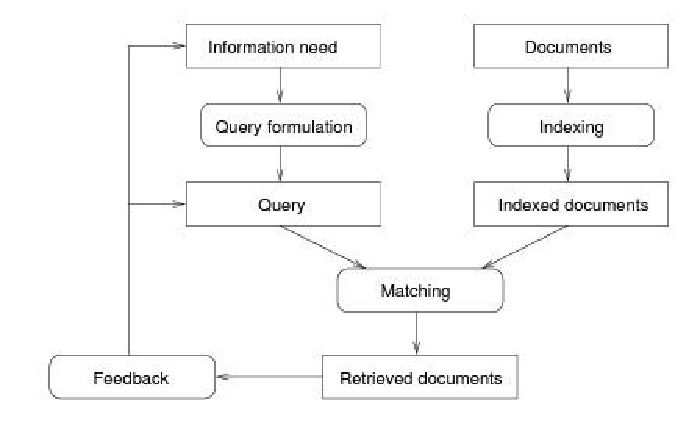
\includegraphics[scale=1.0]{irprocess.pdf}
Aj text môže byť prezentovaný ako obrázok. Stane sa z neho označný plávajúci objekt. Po vytvorení diagramu zrušte znak \texttt{\%} pred príkazom \verb|\includegraphics| označte tento riadok ako komentár (tiež pomocou znaku \texttt{\%}).
\caption{Rozhodujuci argument.}
\label{f:rozhod}
\end{figure*}



\section{Iná časť} \label{ina}

Základným problémom je teda\ldots{} Najprv sa pozrieme na nejaké vysvetlenie (časť~\ref{ina:nejake}), a potom na ešte nejaké (časť~\ref{ina:nejake}).\footnote{Niekedy môžete potrebovať aj poznámku pod čiarou.}

Môže sa zdať, že problém vlastne nejestvuje\cite{bar21health}, ale bolo dokázané, že to tak nie je~\cite{bar21health}. Napriek tomu, aj dnes na webe narazíme na všelijaké pochybné názory\cite{bar21health}. Dôležité veci možno \emph{zdôrazniť kurzívou}.

\section{Ďaľšia časť}
Toto je ďalšia časť, v ktorej idem urobiť odsek.

Toto je odsek. haha.

\subsection{Nejaké vysvetlenie} \label{ina:nejake}

Niekedy treba uviesť zoznam:

\begin{itemize}
\item jedna vec
\item druhá vec
	\begin{itemize}
	\item x
	\item y
	\end{itemize}
\end{itemize}

Ten istý zoznam, len číslovaný:

\begin{enumerate}
\item jedna vec
\item druhá vec
	\begin{enumerate}
	\item x
	\item y
	\end{enumerate}
\end{enumerate}

%\acknowledgement{Ak niekomu chcete poďakovať\ldots}

\bibliography{127323_bibliography}
\bibliographystyle{alpha} %alpha, abbrv
\end{document}
